\chapter{Litreature Review}
\label{ch:intro}
\section{Overview of Relevant Literature}
This chapter presents an overview of relevant literature that underpins the design and development of the proposed localization system. Reviews key techniques in Lidar and LiDAR-Inertial Odometry, SLAM, and localization using a priori maps, with a focus on real-time performance, drift reduction, and global consistency. 
\subsection{LiDAR and LiDAR-Inertial Odometry Techniques}
Localization is a crucial capability for mobile robots, referring to the process of determining the robot’s position and orientation in a given environment. Early attempts at localization depended heavily on wheel encoders, commonly known as wheel odometry, but this method suffered from significant drift whenever the wheels slipped or the ground was uneven \cite{MohamedOdometry}. As robotics advanced, researchers explored range sensors and visual sensors to improve motion estimation \cite{WangVisionSurvey}. At the same time, algorithms like Iterative Closest Point (ICP) emerged, enabling the alignment of consecutive scans and sparking a separate stream of research in range sensor‐based odometry \cite{BeslICP1992}.

Building on these ideas, LiDAR‐only odometry gained popularity due to LiDAR’s immunity to lighting changes and ability to capture dense 3D data. One key approach uses straightforward scan matching via ICP \cite{BeslICP1992}, but such methods can struggle in environments with few unique geometric features. To address this, feature-based systems extract distinctive cues from each LiDAR scan, as demonstrated in LOAM \cite{ZhangSinghLOAM2014}, where sharp edges and planar surfaces guide the matching process. While LiDAR‐only odometry can produce accurate short‐term estimates, it may drift over time if the robot moves rapidly or the environment is mostly repetitive.

To reduce long‐term drift, many researchers incorporate IMU (Inertial Measurement Unit) data, resulting in what is called LiDAR–Inertial Odometry (LIO). In a loosely coupled setup, LiDAR and IMU each compute their own pose, and then a higher‐level filter (like an Extended Kalman Filter) merges these estimates \cite{TangLooselyCoupled}. This approach is easier to design because the LiDAR odometry module and the IMU integration module work somewhat independently. However, the separate modules might not fully exploit each other’s measurements.

By contrast, tightly coupled designs feed raw IMU data directly into the LiDAR optimization. For instance, LIO-SAM employs a factor graph where both LiDAR and IMU “preintegration” factors are updated in the same framework, allowing more constraints to be used in each calculation \cite{ShanEtAlLIOSAM2020}. As graph‐based LiDAR–inertial odometry solutions grew more complex and demanding, researchers began exploring filter‐based methods built around the Kalman filter. One notable example is LINS \cite{lins}, which uses an iterated Error State Kalman filter (iESKF) to speed up pose estimation; however, it still faces performance bottlenecks when dealing with large numbers of LiDAR points, since computing the Kalman gain for every point can be costly. In response, FAST‐LIO \cite{xuFastLIO2021} introduced a more efficient Kalman gain calculation that significantly lowers this overhead. Later, As shown in Figure~\ref{fig:fast_lio2_architecture} FAST‐LIO2 \cite{xuFastLIO2} expanded on that approach by completely removing the feature extraction step and matching raw LiDAR points directly to the map. To accelerate nearest‐neighbor queries, it employs a specialized data structure called an ikd‐Tree, allowing the system to achieve both high accuracy and even faster run.

\begin{figure}
    \centering
    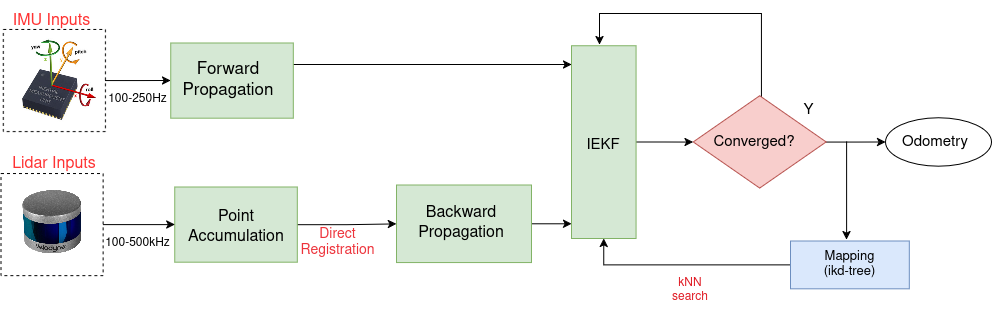
\includegraphics[width=1 \linewidth]{images/fast_lio.drawio.png}
    \caption{Architecture of FAST-LIO2: A tightly coupled LiDAR-Inertial Odometry \cite{yin2021center}}
    \label{fig:fast_lio2_architecture}
\end{figure}

Due to its high computational efficiency, accuracy, and real-time capability, FAST-LIO2 is adopted in this thesis as the LiDAR-Inertial Odometry (LIO) front-end. Its design aligns with the system’s objective to maintain high-frequency odometry while minimizing drift, providing a solid foundation for downstream scan-to-map correction and graph-based fusion.

\subsection{SLAM and Loop Closure-Based Localization}
Moving beyond pure odometry, SLAM (Simultaneous Localization and Mapping) takes an extra step by adding loop closure mechanisms to maintain global consistency \cite{cadena2016past}. While LiDAR–Inertial Odometry can reduce local drift, it remains prone to cumulative error over long distances if no global corrections are made. By detecting revisits to previously mapped areas, a full SLAM pipeline—like Google Cartographer (for 2D LiDAR) \cite{hess2016real} or other graph‐based back ends \cite{grisetti_gmapping}—refines the entire trajectory, resulting in notably higher accuracy. However, these systems carry greater computational cost and design complexity, since maintaining a global graph or submap structure calls for advanced data management. Some research also integrates GNSS (e.g., GPS) data for a global reference frame, further reducing drift when the robot is outdoors. Even then, GNSS signals often fail in heavily built‐up city centers or fully indoor settings, limiting their usefulness for certain applications.

SLAM inherently relies on loop‐closure events or prior constraints to limit its global drift; if these loop closures are sparse or absent over a long trajectory, the system can still accumulate significant positioning errors \cite{grisetti_gmapping, cadena2016past}. That limitation underscores the motivation for map‐based localization, in which an existing map is used to provide absolute constraints and reduce drift, even in lengthy or repetitive environments where loop closures are not guaranteed.

\subsection{Localization Using Prior Maps}
Estimation of the position of a sensor on a map is essential for navigation systems. While several
kinds of map representations are used, depending on the use scenario 3D point cloud maps are among the most popular representations owing to their simplicity and expressiveness.\cite{koide2024tightly}Because constructing a point cloud map is relatively easy with recent precise range sensors and mapping algorithms, point cloud maps are used for a wide range of applications, from indoor service robots to outdoor driving of autonomous vehicles.


Multiple recent works highlight the potential of map-aided localization for achieving robust and precise vehicle pose estimation.\cite{Levinson2007MapBased} propose building a 2D road-surface reflectivity map from lidar data, then using real-time lidar scan correlation against this map to localize within a few decimeters in busy urban areas. Its advantage is straightforward reflectivity matching, but it presupposes consistent road-surface intensity and requires dedicated prior mapping runs.\cite{liu2019segmentation} adopt a detailed segmentation approach: each incoming lidar frame is broken down into ground, curb, edge, and surface features, then aligned with a prior feature map; the refined estimates are further fused with a MEMS-IMU for centimeter-level accuracy at high frequency. Although this improves reliability even in dynamic traffic, the method can become computationally heavy due to multi-type feature extraction and large-scale map management.

By contrast,\cite{Lin2021Autonomous} utilize stereo-based “visual point cloud” maps, avoiding LiDAR hardware yet involving dense stereo matching for both the offline (map) and online (frame) steps. Their system then registers these point clouds via normal distribution transform (NDT). While it lowers sensor costs, it adds a heavy stereo workload and remains susceptible to lighting or texture issues. The authors also report that deviations can occur at sharp turns, albeit these are later corrected. Finally, \cite{Rozenberszki2020LOL} integrate LOAM odometry with a global segment-based prior map (via SegMap) for re-localization when drift accumulates. The system occasionally triggers place recognition in the global map, confirms geometry with RANSAC, then refines the pose using fine-grained ICP. Although segment-based matching proves efficient and effective, it still hinges on stable scene geometry and well-structured offline segmentation.

Overall, these methods demonstrate that leveraging a prior 3D or reflectivity map can curb drift and boost localization accuracy in challenging real-world environments. Still, each approach faces trade-offs in data collection overhead, dynamic scene handling, or computational costs.

\subsection{ Point Cloud Registration Techniques for Localization}
Point cloud registration is a key technique in LiDAR-based localization, used to align a current LiDAR scan with a prior map to estimate the sensor’s pose. The classic Iterative Closest Point (ICP) algorithm performs this by minimizing distances between matched point pairs across the two clouds. While ICP is conceptually simple, it suffers from sensitivity to noise, poor initial alignment, and local minima, making it unreliable for large-scale or noisy environments \cite{BeslICP1992}.\\

To address these limitations, the Normal Distributions Transform (NDT) was proposed by \cite{biber2003ndt} and
further elaborated in subsequent research\cite{magnusson2007ndt}.  NDT offers a compact representation
of surfaces by converting point clouds into a set of local probability density functions
(PDFs), each characterizing a surface section.Instead of relying on discrete point matches, NDT represents the map as a grid of voxels, each containing a Gaussian distribution that models the local geometry. Scan points are registered by maximizing their likelihood under these distributions. This makes NDT more robust to outliers, partial overlaps, and noisy measurements.

Modern implementations such as NDT-OMP further improve runtime performance through multi-threading, enabling real-time scan-to-map matching in large-scale environments \cite{koide2019portable}. Due to its robustness and efficiency, NDT is widely used in autonomous driving and is adopted in this thesis for scan-matching against a pre-built point cloud map.

\subsection{Dynamic Object Removal Techniques for Localization}

In LiDAR-based localization, scan-matching techniques are widely employed to align real-time sensor data with a pre-built static map. However, dynamic objects such as moving vehicles, pedestrians, and cyclists introduce discrepancies between the current point cloud and the static reference. These inconsistencies can significantly degrade localization performance, leading to pose drift, poor convergence, or failure in highly dynamic environments.

To enhance the reliability of scan-matching, dynamic object removal has been introduced as a crucial preprocessing step. Early methods, including Euclidean clustering, geometric filtering, and background subtraction, identified dynamic elements based on heuristics such as size, shape, or temporal consistency \cite{liu2019segmentation,koide2019portable} . Although computationally efficient, these approaches often struggle in cluttered or semi-structured environments, resulting in high false positive rates and poor generalization.
\begin{figure}
	\centering
	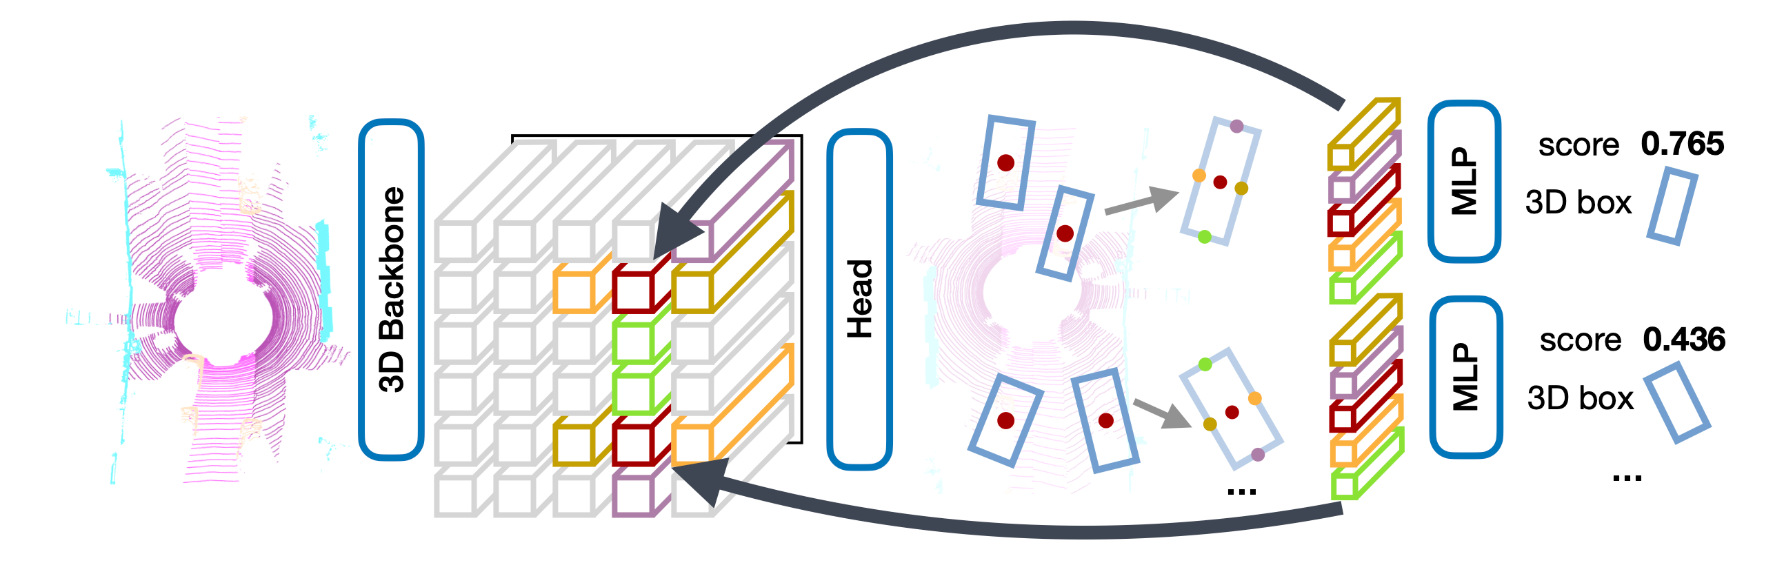
\includegraphics[width=1
	\linewidth]{images/center_point2.png}
	\caption{Overview of CenterPoint 3d object detection framework.  \cite{yin2021center}}
	\label{fig:Overview-CenterPoint }
\end{figure}
Recent advancements leverage deep learning-based 3D object detection models such as PointPillars\cite{lang2019pointpillars}, SECOND \cite{yan2018second}, and CenterPoint \cite{yin2021center} to semantically identify dynamic agents. By predicting 3D bounding boxes for known classes, these models enable precise removal of dynamic objects, preserving static features critical for accurate localization.

Among these, CenterPoint\cite{yin2021center}has emerged as a state-of-the-art solution. It employs a center-based detection paradigm over voxelized LiDAR input and achieves high accuracy on large-scale datasets such as nuScenes\cite{caesar2020nuscenes}, making it particularly suitable for real-time dynamic object filtering.

CenterPoint follows a two-stage architecture\cite{yin2021center}. First, the raw LiDAR point cloud is voxelized into a sparse 3D tensor, allowing efficient processing by sparse convolutional neural networks. A backbone network typically based on PointPillars \cite{lang2019pointpillars} or SECOND\cite{yan2018second} extracts spatial features while maintaining the geometric structure of the environment. These features are projected onto a Bird’s-Eye View (BEV) representation, preserving spatial relationships and enabling faster 2D convolutional operations. In the second stage, a keypoint-based detection head predicts object centers by generating a center heatmap over the BEV feature map. Following center localization, the model regresses the full set of object attributes, including 3D bounding box dimensions, orientation (yaw angle), velocity, and semantic class label. This decoupled center-to-attribute approach simplifies the detection task and enhances robustness against small, distant, or partially occluded objects, as illustrated in Figure \ref{fig:Overview-CenterPoint }.Due to its high detection accuracy and real-time inference capability, CenterPoint is adopted in this work as the dynamic object detection module.



\section{Theoretical Background }
% \subsection{Point-Cloud Registration}

\subsection{Normal Distributions Transform (NDT)}

% \paragraph{Mathematical Formulation}
The NDT algorithm begins by subdividing the space occupied by a scan into discrete grid cells---squares in 2D or cubes in 3D. A PDF is calculated for each cell based on the distribution of points within that cell. Each PDF describes how points within the cell are likely generated, assuming the points result from a multivariate normal random process. The probability density function for a cell is defined as:

\begin{equation}
p(\mathbf{x}) = \frac{1}{(2\pi)^{D/2}|\mathbf{\Sigma}|^{1/2}} \exp\left(-\frac{1}{2}(\mathbf{x}-\mathbf{\mu})^T\mathbf{\Sigma}^{-1}(\mathbf{x}-\mathbf{\mu})\right)
\end{equation}

where $\mu$ and $\Sigma$ denote the mean vector and covariance matrix of the reference of the scan surface points within the cell where x lies. The mean and the covariance are computed as 

\begin{equation}
\mathbf{\mu} = \frac{1}{m} \sum_{k=1}^{m} \mathbf{y}_k
\end{equation}

\begin{equation}
\mathbf{\Sigma} = \frac{1}{m - 1} \sum_{k=1}^{m} (\mathbf{y}_k - \mathbf{\mu})(\mathbf{y}_k - \mathbf{\mu})^T
\end{equation}

where $y_k = 1 ,..., m  \ldots$  are the positions of the reference scan points contained in the cell.

This probabilistic representation gives a piecewise smooth surface approximation with continuous derivatives, capturing the local surface position, orientation, and smoothness effectively.

% \paragraph{Scan Registration Using NDT}
When applying NDT for scan registration, the objective is to determine the pose of the current scan that maximizes the likelihood that scan points align with the reference map surface.The parameters to be optimised; that is, the rotation and translation of the pose estimate of the current scan, can be encoded in a vector $\vec{p}$. The current scan is represented as a point cloud $X = \{\vec{x}_1, \dots, \vec{x}_n\}$. Assume that there is a spatial transformation function $T(\vec{p}, \vec{x})$ that moves a point $\vec{x}$ in space by the pose $\vec{p}$.Given some PDF $\vec{p}$ for scan points, the optimal pose  maximizes the likelihood function:


\begin{equation}
\Psi = \prod_{k=1}^{n} p(T(\mathbf{p}, \mathbf{x}_k))
\end{equation}

or equivalently minimizes the negative log-likelihood of $\Psi$

\begin{equation}
-\log \Psi = -\sum_{k=1}^{n} \log p(T(\mathbf{p}, \mathbf{x}_k))
\end{equation}

    \begin{algorithm}[htbp]
    \caption{Scan Registration using Normal Distributions Transform (NDT)}
    \label{alg:ndt_registration}
    \begin{algorithmic}[1]
        \Require Current scan point cloud $X = \{\vec{x}_1, \dots, \vec{x}_n\}$, Reference map represented by PDFs in grid cells.
        \Ensure Optimized pose vector $\vec{p}$ minimizing negative log-likelihood:
        \[
        -\log \Psi = -\sum_{k=1}^{n} \log p\left(T(\vec{p}, \vec{x}_k)\right)
        \]
    
        \State \textbf{Initialize} pose estimate $\vec{p}$
        \Repeat
        \State Compute objective function:
            \[
            score(\vec{p}) = -\sum_{k=1}^{n}\log p\left(T(\vec{p}, \vec{x}_k)\right)
            \]
        \State Compute gradient and Hessian:
            \[
            \vec{g}(\vec{p}) = \frac{\partial\, score(\vec{p})}{\partial\,\vec{p}}, \quad H(\vec{p}) = \frac{\partial^2\, score(\vec{p})}{\partial\,\vec{p}^2}
            \]
        \State Compute pose update using Newton's method:
            \[
            \Delta\vec{p} = -H(\vec{p})^{-1}\vec{g}(\vec{p})
            \]
        \State Determine step length $\alpha$ (line search):
            \[
            \alpha = \arg\min_{\alpha} score(\vec{p} + \alpha \Delta\vec{p})
            \]
        \State Update pose:
            \[
            \vec{p} \leftarrow \vec{p} + \alpha \Delta\vec{p}
            \]
        \Until{convergence criterion satisfied or maximum iterations reached}
        \State \Return final optimized pose $\vec{p}$
    \end{algorithmic}
    \end{algorithm}

The algorithm for NDT registration is shown in Algorithm \ref{alg:ndt_registration}, The primary distinction between 2D and 3D NDT algorithms resides in the spatial transformation function and its partial derivatives. In 2D, rotations are represented by a single angle, while in 3D, rotations require more complex representations (e.g., rotation matrices or quaternion representations).

\subsection{Sensor Fusion}

\subsubsection{Filtered Based Approaches}
Filtering-based sensor fusion recursively estimates a system’s state (e.g., a robot’s position, orientation, velocity) using two main phases: a prediction step (where the state is propagated using a motion model) and an update step (where incoming sensor measurements refine that prediction) \cite{thrun2005probabilistic}.This real-time, sequential estimation framework is widely employed in robotics to handle noisy sensors while maintaining tractable computational load. Nonetheless, large global corrections or loop closures can be challenging to incorporate without more advanced smoothing or factor-graph techniques\cite{cadena2016past}.

\begin{enumerate}
    \item \textbf{Extended Kalman Filter(EKF) }extends the linear Kalman Filter \cite{kalman1960new} to handle nonlinear systems by linearizing the motion and measurement models around the current estimate.  Let $\mathbf{x}_k$ denote the state at time $k$, and 
    $\hat{\mathbf{x}}_{k|k-1}$ be the predicted mean. 
    
    The \emph{prediction} step is
        \begin{equation}
        \hat{\mathbf{x}}_{k|k-1} = \mathbf{f}\bigl(\hat{\mathbf{x}}_{k-1|k-1}, \mathbf{u}_{k}\bigr), \quad
        \mathbf{P}_{k|k-1} = \mathbf{F}_k \,\mathbf{P}_{k-1|k-1}\,\mathbf{F}_k^T + \mathbf{Q}_k,
        \end{equation}
        where $\mathbf{F}_k$ is the Jacobian of $\mathbf{f}$ w.r.t.\ the state, $\mathbf{Q}_k$ is the process noise covariance, and $\mathbf{u}_k$ is any control input. 
        
    The \emph{update} step uses a measurement model $\mathbf{h}$ is 
        \begin{equation}
        \mathbf{K}_k = \mathbf{P}_{k|k-1} \,\mathbf{H}_k^T 
        \bigl(\mathbf{H}_k\,\mathbf{P}_{k|k-1}\,\mathbf{H}_k^T + \mathbf{R}_k\bigr)^{-1}
        \end{equation}
        \begin{equation}
            \hat{\mathbf{x}}_{k|k} = \hat{\mathbf{x}}_{k|k-1} + \mathbf{K}_k 
            \bigl(\mathbf{z}_k - \mathbf{h}(\hat{\mathbf{x}}_{k|k-1})\bigr),
        \end{equation}
        where $\mathbf{H}_k$ is the Jacobian of $\mathbf{h}$, $\mathbf{R}_k$ is measurement noise covariance, and $\mathbf{z}_k$ is the sensor measurement. The EKF is widely used due to its computational simplicity, although linearization can degrade accuracy in highly nonlinear settings~\cite{thrun2005probabilistic}.
        
    \item \textbf{Error State Kalman Filter(ESKF)} focuses on estimating the \emph{deviation} between a nominal trajectory and the true state~\cite{mourikis2007multi}. A separate routine (e.g., IMU integration) generates a continuous nominal estimate, while the ESKF maintains small \emph{error} states for position, orientation, and sensor biases:
\begin{equation}
\delta \mathbf{x}_k = \mathbf{x}_k - \hat{\mathbf{x}}_{k}^{\text{nominal}}.
\end{equation}
By filtering only $\delta \mathbf{x}_k$, it improves numerical stability in rotation and bias terms, and is particularly effective for high-rate IMU fusion (e.g., in FAST-LIO~\cite{xuFastLIO2021} or LINS~\cite{lins}). Major loop closures or global corrections remain difficult in a strictly forward-update framework~\cite{cadena2016past}.

    \item \textbf{Unscented Kalman Filter(UKF)} avoids explicit Jacobian linearization by employing a deterministic sampling approach (sigma points)~\cite{julier1997new}. A set of points $\{\boldsymbol{\chi}_i\}$ is chosen around the mean and propagated through the nonlinear functions $\mathbf{f}$ and $\mathbf{h}$. The resulting transformed set describes the posterior distribution more accurately than a simple first-order expansion. While the UKF handles significant nonlinearities better than the EKF, it can be more computationally demanding~\cite{thrun2005probabilistic}.

    
\end{enumerate}
% \subsubsection{Factor Graph--Based Sensor Fusion}

% Factor graphs are a powerful framework for multi-sensor fusion in robotics, enabling the simultaneous estimation of all states across time. Unlike filtering approaches such as the Extended Kalman Filter (EKF), factor graphs formulate state estimation as a global optimization problem, naturally handling nonlinearities, drift correction, and loop closures~\cite{cadena2016past, dellaert2017factor}.

% Factor graphs are an undirected bipartite alternative that separate variable nodes (e.g., poses) from factor nodes (e.g., constraints)~\cite{kschischang1998factor}.Figure 2.2 shows a factor graph commonly used in localization and sensor fusion. The green nodes represent robot poses (state variables) over time, while red nodes indicate measurement constraints (e.g., sensor observations) and blue nodes represent motion constraints (e.g., from odometry or IMU). Each factor connects to the relevant states it constrains, forming a graph structure that allows for efficient joint optimization of the trajectory. They explicitly model the factorization of the joint distribution:
% \begin{equation}
% P(X \mid Z) \propto \prod_{k} \phi_k(X_{\alpha(k)}),
% \end{equation}

% where $X$ denotes the entire set of state variables (e.g., poses, sensor biases), and each factor function $\phi_k$ is derived from sensor likelihoods or prior knowledge. The subset $X_{\alpha(k)}$ contains only the variables relevant to factor $k$. When these factors are associated with Gaussian noise models and potentially nonlinear measurement functions, the problem of finding the maximum a posteriori (MAP) estimate translates into a \emph{nonlinear least-squares} problem \cite{cadena2016past, dellaert2017factor}.Figure 

\subsubsection{Factor Graph Based Sensor Fusion}

Factor graphs are a powerful framework for multi-sensor fusion in robotics, enabling the simultaneous estimation of a robot’s trajectory over time. Unlike filtering approaches such as the Extended Kalman Filter (EKF), which operate recursively, factor graphs formulate state estimation as a global optimization problem, making them well-suited for handling nonlinearity, drift correction, and loop closures efficiently~\cite{cadena2016past,dellaert2017factor}.

A factor graph is an undirected bipartite graph that separates variable nodes (e.g., robot poses) from factor nodes (e.g., motion constraints or sensor measurements)~\cite{kschischang1998factor}. As shown in Figure~\ref{fig:factor_graph}, green nodes represent state variables (e.g., the robot’s pose at each time step), while red and blue nodes represent measurement and motion constraints, respectively. Each factor connects only to the variables it influences, forming a sparse, structured representation that is computationally efficient for optimization.

\begin{figure}[ht]
    \centering
    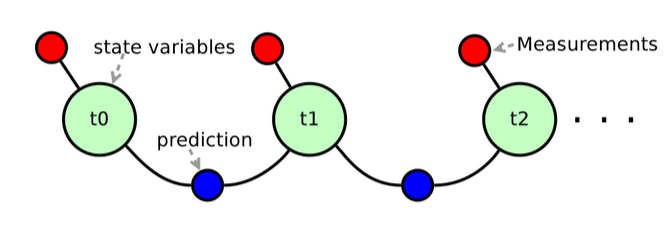
\includegraphics[width=0.7\textwidth]{factor_graph.png}
    \caption{Factor graph representation: green nodes are state variables (poses), blue nodes are motion model factors, and red nodes represent sensor measurements.}
    \label{fig:factor_graph}
\end{figure}

Mathematically, a factor graph models the joint posterior distribution over all states $X$, given observations $Z$, as a product of smaller, local functions:

\begin{equation}
P(X \mid Z) \propto \prod_k \phi_k(X_{\alpha(k)}),
\label{eq:fg_joint}
\end{equation}

where $\phi_k$ is a factor derived from a sensor model or prior, and $X_{\alpha(k)}$ is the subset of state variables relevant to that factor.

In the context of localization, let $X = \{x_0, x_1, \dots, x_n\}$ be the robot’s pose trajectory and $Z = \{z_1, \dots, z_M\}$ be the set of sensor measurements. The joint posterior can be factorized as:

\begin{equation}
P(X \mid Z) \propto P(x_0) \prod_{k=1}^n P(x_k \mid x_{k-1}) \prod_{m=1}^M P(z_m \mid X_{\alpha(m)}),
\label{eq:fg_bayes}
\end{equation}

where:
\begin{itemize}
    \item $P(x_0)$ is the prior on the initial state,
    \item $P(x_k \mid x_{k-1})$ is the motion model (e.g., from IMU preintegration),
    \item $P(z_m \mid X_{\alpha(m)})$ is the sensor measurement model (e.g., LiDAR scan matching).
\end{itemize}

Assuming Gaussian noise, the Maximum A Posteriori (MAP) estimation reduces to a nonlinear least-squares problem:

\begin{equation}
X^* = \arg\min_X \sum_k \| h_k(X_{\alpha(k)}) - z_k \|_{\Sigma_k}^2,
\label{eq:fg_map}
\end{equation}

where $h_k(\cdot)$ is the measurement function, $z_k$ is the observation, and $\Sigma_k$ is the associated noise covariance matrix.


\subsubsection{Incremental Solvers and Real-Time Performance}
For real-time or large-scale applications, solving the entire problem from scratch at each step may be intractable \cite{thrun2005probabilistic}. Incremental smoothing algorithms like iSAM2 \cite{kaess2012isam2} maintain a factorization of the problem in a data structure (often a Bayes tree) that can be efficiently updated with new measurements. Rather than re-solving globally each time, iSAM2 carries out local re-linearization and partial variable reordering, providing near-constant-time updates for many practical cases.

